\documentclass[final,xcolor=table,svgnames]{beamer}
\usepackage[english]{babel}
%\usepackage[latin1]{inputenc}
\usepackage[T1]{fontenc}
\usepackage{graphicx}
\usepackage{hyperref}
\usepackage{url}
\usepackage{tikz}
\usepackage{doi}
\usepackage{booktabs}
\usepackage{fontawesome}
\usepackage{academicons}
\usepackage{fontspec}
\usepackage{colortbl}


\setmainfont{Gillius ADF No2}

\newcommand{\logoheight}{1cm}

\DeclareGraphicsExtensions{.pdf,.png,.PNG,.JPG,.jpg,.jpeg,.gif}
\graphicspath{
{./figures/},
{./figures/scientificprofiles/}
{/home/ctroupin/Presentations/figures4presentations/logo/},
}


\setbeamertemplate{navigation symbols}{}
\setbeamertemplate{items}[square] 
\setbeamertemplate{caption}[numbered]
%\setbeamerfont{caption}{size=\scriptsize,family=\it}

%\usefonttheme{professionalfonts} % using non standard fonts for beamer
%\usefonttheme{serif} % default family is serif

\usetikzlibrary{arrows,shapes,backgrounds}
\tikzstyle{every picture}+=[remember picture]
\tikzstyle{na} = [baseline=-.5ex]

\definecolor{bluegher}{HTML}{4E519F}
\definecolor{mygrey}{rgb}{0.75,.75,.75}
\definecolor{arrowcolor}{rgb}{0.1,0.1,0.1}
\definecolor{alertbg}{HTML}{FEFFBA}

\setbeamercolor{title}{fg=white}
\setbeamercolor{institute}{fg=mygrey}
\setbeamercolor{frametitle}{fg=white,bg=bluegher}
\setbeamercolor{structure}{fg=bluegher}
\setbeamercolor{item projected}{fg=black}
\setbeamercolor{alerted text}{fg=bluegher,bg=alertbg}

\setbeamercovered{invisible}
\setbeamertemplate{items}[triangle] 

\newenvironment{boxalertenv}{\begin{altenv}%
      {\usebeamertemplate{alerted text begin}\usebeamercolor[fg]{alerted text}\usebeamerfont{alerted text}\colorbox{bg}}
      {\usebeamertemplate{alerted text end}}{\color{.}}{}}{\end{altenv}}

\newcommand<>{\boxalert}[1]{{%
  \begin{boxalertenv}#2{#1}\end{boxalertenv}%
}}


\setbeamerfont{sectiontitle1}{size=\huge,family=\rmfamily}
\setbeamerfont{sectiontitle2}{size=\fontsize{40}{20}\selectfont,shape=\itshape,family=\rmfamily}
\setbeamerfont{author}{size=\large,family=\rmfamily}
\setbeamerfont{institute}{size=\normalsize,family=\rmfamily}
\setbeamerfont{title}{size=\fontsize{25}{20}\selectfont,shape=\itshape,family=\rmfamily}

\setbeamertemplate{enumerate items}[square]
\setbeamercolor{item projected}{bg=alertbg,fg=bluegher}

\setbeamertemplate{title page}{%
\begin{tikzpicture}[remember picture,overlay]
\fill[bluegher]
  (current page.west) rectangle (current page.south east);
\node[anchor=east] 
  at ([yshift=-30pt, xshift=-10pt]current page.north east) (author)
  {\parbox[t]{.6\paperwidth}{\raggedleft%
   \usebeamerfont{author}{\insertauthor}}};
\node[anchor=north east] 
  at ([yshift=-70pt, xshift=-10pt]current page.north east) (institute)
  {\parbox[t]{.78\paperwidth}{\raggedleft%
    \usebeamerfont{institute}\usebeamercolor[fg]{institute}{\insertinstitute}}};
\node[anchor=south west] 
  at ([yshift=20pt, xshift=20pt]current page.west) (logo)
  {\parbox[t]{.19\paperwidth}{\centering%
    \usebeamercolor[fg]{titlegraphic}\inserttitlegraphic}};
\node[anchor=east]
  at ([yshift=-55pt,xshift=-20pt]current page.east) (title)
  {\parbox[t]{\textwidth}{\raggedleft%
   \usebeamerfont{title}\usebeamercolor[fg]{title}\inserttitle}};
\end{tikzpicture}
}

%\setbeamersize{text margin left=1cm}

\newlength{\logoH}
\setlength{\logoH}{1cm}
\newcommand{\montant}{\rule{0pt}{3ex}}

%--------------------------------
\hypersetup{bookmarksopen=true,
bookmarksnumbered=true,  
pdffitwindow=true, 
pdfstartview=Fit,
%pdfpagemode=FullScreen,
pdffitwindow=true,
pdftoolbar=true,
pdfmenubar=true,
pdfwindowui=true,
pdfsubject={ODIP, Data analysis, Software citation},
pdfauthor={C. Troupin, C. Muñoz, S. Watelet, A. Barth, J.M. Beckers},
bookmarksopenlevel=0,
colorlinks=true,
linkcolor=bluegher,anchorcolor=black,%
citecolor=bluegher,filecolor=black,%
menucolor=black,urlcolor=bluegher,%
pdfpageduration=1,%
}


\title{Software citation \& \newline process traceability}
%\subtitle{}
\author[C.~Troupin]{C.~Troupin$^{\star}$, C.~Muñoz$^{\ast}$,\\S.~Watelet$^{\star}$, A.~Barth$^{\star}$ \& J.-M.~Beckers$^{\star}$}

\institute{$^{\star}$GHER-University of Liège

$^{\ast}$Balearic Islands Coastal Ocean\\ Observing and Forecasting System}

\date{Galway (Ireland), 2-6 October, 2017}
\titlegraphic{\includegraphics[height=\logoheight]{logo_odip2}
\includegraphics[height=\logoheight]{logo_uliege.jpeg}\\
\includegraphics[height=\logoheight]{logo_gher}
\includegraphics[height=\logoheight]{logo_socib}}
 
 \tikzset{
    vertex/.style = {
        circle,
        fill = black,
        outer sep = 0pt,
        inner sep = 1pt,
    }
}

\begin{document}

\begin{frame}
\maketitle
\end{frame}

%--------------------------------------------------------------------------------------------------------------
\begin{frame}
\frametitle{Persistent identifier everywhere}
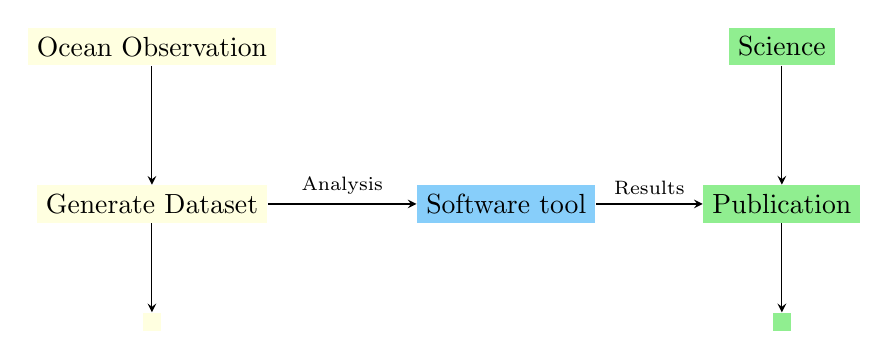
\begin{tikzpicture}

%\node[anchor=south west,inner sep=0] (image) at (0,0) {\includegraphics[width=0.9\textwidth]{figures/im_back.png}};
     
%\draw[help lines,xstep=1,ystep=1] (0,0) grid (10,10);
%\foreach \x in {0,1,...,9} { \node [anchor=north] at (\x,0) {\x}; }
%\foreach \y in {0,1,...,9} { \node [anchor=east] at (0,\y) {\y}; }

\onslide<1->{
\node[fill=LightYellow,text=black] (OceanObservation)  at (1,7) {Ocean Observation};
\node[fill=LightGreen,text=black] (Science) at (9,7) {Science};

}

\onslide<2->{
\node[fill=LightYellow,text=black] (GenerateDataset) at (1,5) {Generate Dataset};
\draw[->,>=stealth] (OceanObservation) edge (GenerateDataset);
}

\onslide<3->{
\node[fill=LightSkyBlue,text=black] (Software) at (5.5,5) {Software tool};
\node[fill=LightGreen,text=black] (Publication) at (9,5) {Publication};
\draw[->,>=stealth] (Science) edge (Publication);
\draw[->,>=stealth] (GenerateDataset) edge node[anchor=center, above] {\scriptsize Analysis} (Software);
\draw[->,>=stealth] (Software) edge node[anchor=center, above] {\scriptsize Results} (Publication);
}

\onslide<4->{
\node[fill=LightYellow,text=black] (DOIdata) at (1,3.5) {\aiDoi};
\node[fill=LightGreen,text=black] (DOIpub) at (9,3.5) {\aiDoi};
\draw[->,>=stealth](GenerateDataset) edge (DOIdata);
\draw[->,>=stealth](Publication) edge (DOIpub);
}
 
\end{tikzpicture}


\onslide<5>{
How can we ensure the readers/users\\
 can \alert{reproduce} the results?
}

\end{frame}


%-----------------------------------------------------------------------------------------------
\section{Software citation}
\begin{frame}[c]

\begin{tikzpicture}[remember picture,overlay]
\fill[bluegher]
  (current page.west) rectangle (current page.south east);
\node[anchor=east] 
  at ([yshift=35pt, xshift=-20pt]current page.east) (title1)
  {\parbox[t]{.6\paperwidth}{\raggedleft%
   \usebeamerfont{sectiontitle1}{Persistent identifiers:\\
what about}}};
\node[anchor=east]
  at ([yshift=-35pt,xshift=-20pt]current page.east) (title2)
  {\parbox[t]{\textwidth}{\raggedleft%
   \usebeamerfont{sectiontitle2}\usebeamercolor[fg]{title}{software tools?}}};
\end{tikzpicture}
\end{frame}



%-----------------------------------------------------------------------------------------------

\begin{frame}
\frametitle{Context: who has done what, and how?}

\onslide<2>{Let's work with ORCID}\\[1cm]



\centering
\huge 
\aiAcademia
\aiAcclaim
\aiACM
\aiADS
\aiarXiv
\aibioRxiv
\aiCEUR
\aiCoursera
\aidblp
\aiDepsy

\aiDoi
\aiDryad
\aiFigshare
\aiGoogleScholar
\aiIEEE
\aiImpactstory
\aiInspire
\aiMendeley
\aiOpenAccess
\alert<2>{\aiOrcid}

\aiOSF
\aiOverleaf
\aiPhilPapers
\aiPiazza
\aiPublons
\aiPubMed
\aiResearchGate
\aiSciRate
\aiSpringer
\aiZotero

{\footnotesize Source: \href{http://jpswalsh.github.io/academicons/}{Academicons}}

\end{frame}
%-----------------------------------------------------------------------------------------------

\begin{frame}[c]
\frametitle{Data and data sets identification citation}

\onslide*<1>{
See previous ODIP workshops + links to other initiatives 
\begin{itemize}
\item[] \href{https://www.rd-alliance.org/groups/data-citation-wg.html}{Research Data Alliance} Data Citation working group
\item[] \href{http://www.project-thor.eu/}{THOR project}
\item[] \href{https://www.pangaea.de/}{Pangaea}
\end{itemize}

\begin{figure}
\centering
\includegraphics[width=.6\textwidth]{MedGibData}
\end{figure}
}

\onslide*<2>{Data set in peer-reviewed journals 

\begin{itemize}
\item[] \href{http://www.earth-syst-sci-data.net}{Earth System Science Data}\\
"\textit{\footnotesize reuse of high-quality data of benefit to Earth system sciences}"\\
30 articles in 2017 (as of July 24th)
\item[] \href{https://www.nature.com/sdata/}{Scientific Data}\\
"\textit{\footnotesize promote wider data sharing and reuse, and to credit those that share}"\\
106 publications in 2017 (all disciplines)
\end{itemize}
}

\end{frame}

%-----------------------------------------------------------------------------------------------

\begin{frame}
\frametitle{Products and results}

\onslide*<1>{
\textbf{Results=} \\
numerical model outputs (re-analysis, forecasts)\\
climatologies build from in situ data\\
aggregated datasets

\vspace{1cm}

\textbf{Goals:} \\
proper citation in publications\\
control of different versions of the same product
}

\onslide*<2>{
\textbf{Example:} SeaDataNet Product Catalog (\href{http://sextant.ifremer.fr/en/web/seadatanet/}{Sextant})\\
Mediterranean Sea: Temperature and Salinity Climatology V1.1

\begin{figure}
\centering
\includegraphics[width=.95\textwidth]{sextant_medsea}
\end{figure}

\begin{itemize}
\footnotesize
\item Internal permanent shortname: {\texttt 90ae7a06-8b08-4afe-83dd-ca92bc99f5c0}
\item DOI: \href{http://dx.doi.org/10.12770/90ae7a06-8b08-4afe-83dd-ca92bc99f5c0}{10.12770/90ae7a06-8b08-4afe-83dd-ca92bc99f5c0}
\end{itemize}
}

\onslide*<3>{

% A new version of such a product (climatology) would happen if the aggregated data set is updated or if another version of the software is employed. 
\begin{figure}
\centering
\begin{tikzpicture}[spy using outlines={rectangle,red,magnification=5,width=8.cm,height=1cm, connect spies}]
\node[anchor=south west,inner sep=0] (image) at (0,0) {\pgfimage[interpolate=true,width=.7\textwidth]{figures/sextant_medsea3.png}};

\begin{scope}[x={(image.south east)},y={(image.north west)}]
    %\draw[help lines,xstep=.1,ystep=.1] (0,0) grid (1.2,1.2);
    %\foreach \x in {0,1,...,12} { \node [anchor=north] at (\x/10,0) {0.\x}; }
    %\foreach \y in {0,1,...,12} { \node [anchor=east] at (0,\y/10) {0.\y}; }
    \coordinate (center) at (.44, .43);
    \coordinate (pos spy) at (.65,.15);
\onslide<2->{\spy on (center) in node [] at (pos spy);}
\end{scope}

\end{tikzpicture}
\end{figure}

Can we go further and have:\\
"\textit{The version used for the DIVA software is the 4.6.9,\\
doi: \href{http://dx.doi.org/10.5281/zenodo.836727}{10.5281/zenodo.836727}}"
?
}

\end{frame}

%-----------------------------------------------------------------------------------------------

\begin{frame}
\frametitle{Software tools and methods: journals}

\onslide*<1>{
\href{https://www.geoscientific-model-development.net/)}{Geoscientific Model Development}
\begin{itemize}
\footnotesize 
\it
\item "description, development, and evaluation of numerical models\\ of the Earth system and its components"
\item "geoscientific model descriptions, from statistical models\\ to box models to GCMs"
\item "Inclusion of Code and/or data availability sections\\ is mandatory for all papers"
%"May include a \textbf{user manual} and actual \textbf{code} (as supplementary information)."
%"Submission of short papers describing subsequent model development and \textbf{bug-fixes} will be encouraged."
\end{itemize}


\begin{figure}
\centering
\includegraphics[width=.8\textwidth]{GMD_divand}\\
\scriptsize \doi{10.5194/gmd-7-225-2014}
\end{figure}
}

\onslide*<2>{
\href{https://link.springer.com/journal/12145}{Earth Science Informatics}
\begin{itemize}
\footnotesize 
\it 
\item "(...) cutting-edge, and provocative scientific work\\ in the area of Earth Science Informatics (...)"
\item "(...) all aspects of computer applications to the acquisition, storage, processing, interchange, and visualization of data"
\item Sub-disciplines: Ontology, Simulation and Modeling, Information Systems Applications
\end{itemize}

\begin{figure}
\centering
\includegraphics[width=.8\textwidth]{Esin_paper}\\
\scriptsize \doi{10.1007/s12145-016-0266-2}
\end{figure}
}

\onslide*<3>{
\href{https://www.journals.elsevier.com/methods-in-oceanography}{Methods in Oceanography}
\begin{itemize}
\footnotesize 
\it 
\item "original research on new methods in all aspects of oceanographic research"
\item "significant advances in the development of new methods for the interpretation of either existing or future data"
\end{itemize}

\begin{figure}
\centering
\includegraphics[width=.8\textwidth]{Mio_paper}\\
\scriptsize \doi{10.1016/j.mio.2016.05.001}
\end{figure}

{\scriptsize \faBomb discontinued as of 2017}

}






\end{frame}

%-----------------------------------------------------------------------------------------------
\section{Notebooks}

\begin{frame}[c]

\begin{tikzpicture}[remember picture,overlay]
\fill[bluegher]
  (current page.west) rectangle (current page.south east);
\node[anchor=east] 
  at ([yshift=35pt, xshift=-20pt]current page.east) (title1)
  {\parbox[t]{.6\paperwidth}{\raggedleft%
   \usebeamerfont{sectiontitle2}{Notebooks}}};
\node[anchor=east]
  at ([yshift=-35pt,xshift=-20pt]current page.east) (title2)
  {\parbox[t]{\textwidth}{\raggedleft%
   \usebeamerfont{sectiontitle1}\usebeamercolor[fg]{title}{for documenting work-flows
}}};
\end{tikzpicture}

\end{frame}






\end{document}



%-----------------------------------------------------------------------------------------------
\begin{frame}[t]
\frametitle{Where is the data?}

\begin{columns}[T]
\begin{column}{0.6\textwidth}
\begin{itemize}
\item<1-> Institutional portals
\item<2-> International portals
\item<3-> Paper + portal 
\item<4-> Personal disk?
\end{itemize}

\end{column}
\begin{column}{0.4\textwidth} 
\onslide*<1>{
\includegraphics[width=.85\columnwidth]{Corioliscatalog}

\includegraphics[width=.85\columnwidth]{AODNcatalog.png}

\includegraphics[width=.85\columnwidth]{SOCIBcatalog}
}
\onslide*<2>{
\includegraphics[width=.85\columnwidth]{SeaDataNet}

\includegraphics[width=.85\columnwidth]{EMODnet}

\includegraphics[width=.85\columnwidth]{CMEMScatalog}
}

\onslide*<3>{\footnotesize
\doi{10.5194/essd-8-141-2016}\\
\includegraphics[width=.85\columnwidth]{MedGibPaper}
\vspace{.5cm}
\doi{10.1594/PANGAEA.853701}\\
\includegraphics[width=.85\columnwidth]{MedGibData}


}
\onslide*<4>{\includegraphics[width=.9\columnwidth]{results.jpg}}
\end{column}
\end{columns}
\end{frame}



%-----------------------------------------------------------------------------------------------
\begin{frame}[t]
\frametitle{Where are the results/products?}

\begin{columns}[T]
\begin{column}{0.45\textwidth}
\begin{itemize}
\item<2-> Personal disks
\item<3-> Product catalog
\item<4-> Web page + PDF reports to be cited
\end{itemize}
\vspace{1cm}

\onslide*<3>{\footnotesize DOI not always used, but rather an "Internal permanent shortname"\\
ex: 4b65b074-19a2-11e5-95c0-8056f28224bb
}

\end{column}
\begin{column}{0.55\textwidth} 
\onslide*<2>{
\includegraphics[width=.9\columnwidth]{results.jpg}
}

\onslide*<3>{
\includegraphics[width=.9\columnwidth]{EMODnetChemCatalog}
\vspace{.5cm}
\includegraphics[width=.9\columnwidth]{SextantCatalog}
}

\onslide*<4>{ 
\footnotesize World Ocean Atlas\\
\url{https://www.nodc.noaa.gov/OC5/woa13/}\\
\includegraphics[width=.9\columnwidth]{WOAcatalog}
\vspace{.5cm}
\includegraphics[width=.9\columnwidth]{WOApub}
}

\end{column}
\end{columns}

\end{frame}

%-----------------------------------------------------------------------------------------------
\begin{frame}[t]
\frametitle{How to go from data to products?}

\begin{columns}[T]
\begin{column}{0.45\textwidth}
\begin{itemize}
\item<1-> Read the publication?
\item<2-> Read the manual?
\item<3-> Get linked code from publication
\end{itemize}

\end{column}
\begin{column}{0.55\textwidth} 
\onslide*<1>{
\includegraphics[width=.9\columnwidth]{paperread}
}

\onslide*<2>{
\includegraphics[width=.9\columnwidth]{RTFM_Whiteboard}

\includegraphics[width=.9\columnwidth]{RTFM2.jpg}
}

\onslide*<3>{\footnotesize \doi{10.5194/gmd-10-765-2017}\\
\includegraphics[width=.9\columnwidth]{PaperCode}

\doi{10.5194/gmd-7-225-2014}\\
\includegraphics[width=.9\columnwidth]{DivandPaper}
}


\end{column}
\end{columns}

\end{frame}

%------------------------------------------------------------------------------------------------

\begin{frame}
\frametitle{A closer look to Zenodo}

\onslide*<1>{\includegraphics[width=.8\textwidth]{zenodo1}}
\onslide*<2>{\includegraphics[width=.8\textwidth]{zenodo2}}
\onslide*<3>{\includegraphics[width=.8\textwidth]{zenodo4}}

\vspace{.5cm}


\onslide*<1>{Allows loggin with \textbf{GitHub} or \textbf{ORCID}}
\onslide*<2>{Allows linking accounts with \textbf{GitHub} and \textbf{ORCID}}
\onslide*<3>{Anything can be uploaded and cited}
\end{frame}

%------------------------------------------------------------------------------------------------

\begin{frame}
\frametitle{Generating DOI for software releases}

\onslide*<1>{\includegraphics[width=.85\textwidth]{zenodo3}}
\onslide*<2>{\includegraphics[width=.85\textwidth]{github1}}
\onslide*<3>{\includegraphics[width=.85\textwidth]{github3}}
\onslide*<4>{\includegraphics[width=.85\textwidth]{github_release1}}
\onslide*<5>{\includegraphics[width=.85\textwidth]{github_release2}}
\onslide*<6>{\includegraphics[width=.85\textwidth]{github_release3}}
\onslide*<7>{\includegraphics[width=.85\textwidth]{github_release4}}
\onslide*<8>{\includegraphics[width=.85\textwidth]{zenodo_release}}
\onslide*<9>{\includegraphics[width=.85\textwidth]{zenodo_release2}}

\vspace{.5cm}

\onslide*<1>{Select \textbf{GitHub} repositories to be synced with Zenodo}
\onslide*<2>{Go on your GitHub home page}
\onslide*<3>{In settings: allow third-party access}
\onslide*<4>{Open the project repository}
\onslide*<5>{Click on the \textit{Release} button}
\onslide*<6>{Fill in the information and \ldots}
\onslide*<7>{\ldots make the release}
\onslide*<8>{Check the project release on Zenodo and \ldots}
\onslide*<9>{\ldots get the DOI badge}
\end{frame}

%------------------------------------------------------------------------------------------------


\begin{frame}[t]
\frametitle{Use-case: Diva releases}

\begin{enumerate}
\item<1-> Switch from SVN to GitHub (conserving the history) 
\item<2-> Enable Diva repository on Zenodo
\item<3-> Edit the different \textit{tags} on GitHub (otherwise DOI not generated) 
\item<4-> To do? Include Diva corresponding DOI in product netCDF?
\end{enumerate}
\vspace{1cm}

\onslide*<1>{\footnotesize
Resources:
\begin{itemize}
\item \url{https://git-scm.com/book/en/v2/Git-and-Other-Systems-Migrating-to-Git}
\item \url{http://john.albin.net/git/convert-subversion-to-git}
\item \url{https://www.atlassian.com/git/tutorials/migrating-overview}
\end{itemize}
}

\onslide*<2>{
\includegraphics[width=.75\textwidth]{zenodoDiva}
}

\onslide*<3>{
\includegraphics[width=.75\textwidth]{zenodoDiva2}
}


\end{frame}

%------------------------------------------------------------------------------------------------



\end{document}
